\documentclass{beamer}

\usepackage[T1]{fontenc}
\usepackage[utf8]{inputenc}
\usepackage[slovene]{babel}
\usepackage{hyperref}
\usepackage{tikz}

\usepackage{palatino}
\usefonttheme{serif}

\setbeameroption{hide notes}
\mode<presentation>
\usetheme[secheader]{Madrid}

\setbeamertemplate{navigation symbols}{}
% ===================================================================
\begin{document}
\title{Priprava prosojnic v {\LaTeX}-u}
\subtitle{Uporaba paketa \texttt{beamer}}
\author{Jon Mikoš}
\institute[FMF]{Fakulteta za matematiko in fiziko}
\date{}

\begin{frame}
   \titlepage
\end{frame}
% -------------------------------------------------------------------
\begin{frame}
   \frametitle{Kratek pregled}
   \tableofcontents
\end{frame}
% ===================================================================
\section{Razporeditev vsebine}
% -------------------------------------------------------------------
\begin{frame}
   \frametitle{Naštevanje}
   Za naštevanje lahko uporabimo okolje \texttt{itemize}:
   \begin{itemize}
      \item Prva točka.
      \item Druga točka.
      \item Tretja točka.
   \end{itemize}
   ali pa okolje \texttt{enumerate}:
   \begin{enumerate}
      \item Prva točka.
      \item Druga točka.
      \item Tretja točka.
   \end{enumerate}
\end{frame}
% -------------------------------------------------------------------
\begin{frame}
   \frametitle{Bloki z naslovom}
   Dele besedila lahko zapišemo v bloke.\\
   Uporabimo okolja \texttt{block}, \texttt{exampleblock}, \texttt{alertblock}.\\
   Za parameter okolja napišemo naslov bloka.\\
   \begin{block}{Opomba}
      Tako je videti block z naslovom.
   \end{block}
   \begin{exampleblock}{Primer}
      Tako je videti exampleblock z naslovom.
   \end{exampleblock}
   \begin{alertblock}{Opozorilo}
      Tako je videti alertblock z naslovom.
   \end{alertblock}
\end{frame}
% -------------------------------------------------------------------
\begin{frame}
   \frametitle{Bloki brez naslova}
   Blok lahko ima tudi prazen naslov.\\
   V takem primeru bo brez naslovne vrstice.
      \begin{block}{}Tako je videti \texttt{block} s praznim naslovom.\end{block}
      \begin{exampleblock}{}Tako je videti \texttt{exampleblock} s praznim naslovom.\end{exampleblock}
      \begin{alertblock}{}Tako je videti \texttt{alertblock} s praznim naslovom.\end{alertblock}
\end{frame}
% -------------------------------------------------------------------
\begin{frame}
   \frametitle{Stolpci}
      \begin{columns}
         \begin{column}{0.5\textwidth}
            \begin{itemize}
               \item Besedilo lahko pišemo v več stolpcih.
               \item Osnovno okolje je columns.
               \item Posamezen stolpec opišemo v okolju column.
               \item Vsebina stolpca je lahko poljubna.
               \item Za primer imamo v desnem stolpcu napis v bloku in sliko sončnice.
            \end{itemize}
         \end{column}
         \begin{column}{0.5\textwidth}
            \begin{exampleblock}{}
               Slika v stolpcu.
            \end{exampleblock}
            \includegraphics{soncnica.jpg}
         \end{column}
      \end{columns}
\end{frame}
% ===================================================================

\section{Matematične trditve}

% -------------------------------------------------------------------
\begin{frame}
   \frametitle{Praštevila}
   \begin{block}{Definicija}
      \emph{Praštevilo je naravno število, ki ima natanko dva delitelja.}
   \end{block}
   \begin{exampleblock}{Zgledi}
      \begin{itemize}
         \item 1 je praštevilo (ima samo enega delitelja: 1).
         \item 2 je praštevilo (ima dva delitelja: 1 in 2).
         \item 3 je praštevilo (ima dva delitelja: 1 in 3).
         \item 4 ni praštevilo (ima tri delitelje: 1, 2 in 4).
      \end{itemize}
   \end{exampleblock}
\end{frame}
% -------------------------------------------------------------------
\begin{frame}
   \frametitle{Praštevila}
   \begin{block}{Izrek}
      \emph{Praštevil je neskončno mnogo.}
   \end{block}
   \begin{block}{Dokaz.}
      Denimo, da je praštevil končno mnogo.
      \begin{itemize}
         \item Naj bo $p$ največje praštevilo.
         \item Naj bo $q$ produkt števil $1, 2, \dots , p$.
         \item Število $q+1$ ni deljivo z nobenim praštevilom, torej je $q+1$ praštevilo.
         \item To je protislovje, saj je $q+1>p$.
      \end{itemize}
   \end{block}
\end{frame}
% ===================================================================

\section{Postopno odkrivanje vsebine}

% -------------------------------------------------------------------
\begin{frame}
   \frametitle{Konstrukcija pravokotnice na premico p skozi točko T}
   \begin{columns}
      \begin{column}{0.5\textwidth}
         \begin{itemize}
            \visible<1->{\item Dani sta premica p in točka T.}
            \visible<2->{\item Nariši lok k s središčem v T.}
            \visible<3->{\item Premico p seče v točkah A in B.}
            \visible<4->{\item Nariši lok m s središčem v A.}
            \visible<5->{\item Nariši lok n s središčem v B in z enakim polmerom.}
            \visible<6->{\item Loka se sečeta v točki C.}
            \visible<7->{\item Premica skozi točki T in C je pravokotna na p.}
         \end{itemize}
      \end{column}
      \begin{column}{0.5\textwidth}
         \begin{figure}
            \includegraphics<1>[width=\textwidth]{pic1.png}
            \includegraphics<2>[width=\textwidth]{pic2.png}
            \includegraphics<3>[width=\textwidth]{pic3.png}
            \includegraphics<4>[width=\textwidth]{pic4.png}
            \includegraphics<5>[width=\textwidth]{pic5.png}
            \includegraphics<6>[width=\textwidth]{pic6.png}
            \includegraphics<7>[width=\textwidth]{pic7.png}
         \end{figure}
      \end{column}
   \end{columns}
\end{frame}
% -------------------------------------------------------------------
\begin{frame}
   \frametitle{Odkrivanje tabele po vrsticah}
   \begin{columns}
      \begin{column}{0,5\textwidth}
         \begin{table}
            \begin{tabular}{c|*{4}{c}}
            \visible<1->{Oznaka & A & B & C & D \\\hline}
            \visible<2->{X      & 1 & 2 & 3 & 4 \\      }
            \visible<3->{Y      & 3 & 4 & 5 & 6 \\      }
            \visible<4->{Z      & 5 & 6 & 7 & 8         }
            \end{tabular}
         \end{table}
      \end{column}
      \begin{column}{0,5\textwidth}
      \end{column}
   \end{columns}
\end{frame}
% -------------------------------------------------------------------
\begin{frame}
   \frametitle{Odkrivanje tabele po stolpcih}
   \begin{columns}
      \begin{column}{0.5\textwidth}
         \begin{table}
            \begin{tabular}{c|*{4}{c}}
            \visible<1->{Oznaka} & \visible<2->{A} & \visible<3->{B} & \visible<4->{C} & \visible<5->{D} \\\hline
            \visible<1->{X     } & \visible<2->{1} & \visible<3->{2} & \visible<4->{3} & \visible<5->{4} \\
            \visible<1->{Y     } & \visible<2->{3} & \visible<3->{4} & \visible<4->{5} & \visible<5->{6} \\
            \visible<1->{Z     } & \visible<2->{5} & \visible<3->{6} & \visible<4->{7} & \visible<5->{8} \\
            \end{tabular}
         \end{table}
      \end{column}
      \begin{column}{0.5\textwidth}
      \end{column}
   \end{columns}
\end{frame}
% ===================================================================

\section{Razno}

% -------------------------------------------------------------------
\begin{frame}
   \centering
   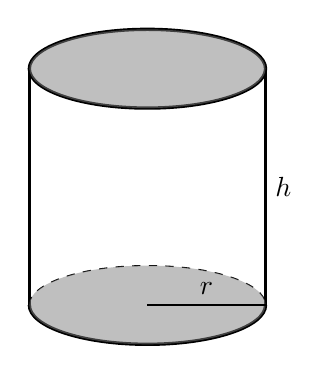
\begin{tikzpicture}
      \draw [very thick] (0,0) ellipse (1.5 and 0.5);
      \draw [very thick] (-1.5,0) -- (-1.5,-3);
      \draw [very thick] (-1.5,-3) arc (180:360:1.5 and 0.5);
      \draw [dashed] (-1.5,-3) arc (180:360:1.5 and -0.5);
      \draw [very thick] (1.5,-3) -- (1.5,0);
      \visible<2->{\fill [gray, opacity=0.5] (0,0) ellipse (1.5 and 0.5);}
      \visible<2->{\fill [gray, opacity=0.5] (-1.5,-3) arc (180:360:1.5 and -0.5) -- (-1.5,-3) arc (180:360:1.5 and 0.5);}
      \visible<3->{\draw [thick] (0,-3) -- (1.5,-3) node[pos=0.5, above] {$r$};}
      \visible<3->{\node[right] at (1.5,-1.5) {$h$};}
   \end{tikzpicture}
\end{frame}
% ===================================================================
\end{document}
